\documentclass[12pt,a4paper,twoside]{article}

% Packages
\usepackage[margin=1in]{geometry}
\usepackage{cite}
\usepackage{amsmath,amssymb,amsfonts}
\usepackage{graphicx}
\usepackage{textcomp}
\usepackage{xcolor}
\usepackage[hidelinks]{hyperref}
\usepackage{listings}
\usepackage{titlesec}
\usepackage{tikz}
\usepackage{booktabs}
\usepackage{float}
\usepackage{fancyhdr}
\usepackage[font=small,labelfont=bf]{caption}
\usepackage{subcaption}
\usepackage{algorithm}
\usepackage{algpseudocode}
\usepackage{tocloft}
\usetikzlibrary{shapes.geometric, arrows.meta, positioning, calc, fit}

% Reduce TOC spacing to fit on fewer pages
\setlength{\cftbeforesecskip}{2pt}
\setlength{\cftbeforesubsecskip}{1pt}

% Graphics path - figures are stored in results/figures
\graphicspath{{../results/figures/}{figures/}}

% Header/footer setup
\pagestyle{fancy}
\fancyhf{}
\fancyhead[LE]{Reinforcement Learning Applied to the Snake Game}
\fancyhead[RO]{Al-Amri, Al-Ubejdij, Al-Moslemani, Humaid, Aldous, Gavankar}
\fancyfoot[C]{\thepage}
\renewcommand{\headrulewidth}{0.4pt}

% No paragraph indentation
\setlength{\parindent}{0pt}
\setlength{\parskip}{6pt}

% Prevent LaTeX from stretching vertical space to fill pages
\raggedbottom

% Document metadata
\def\BibTeX{{\rm B\kern-.05em{\sc i\kern-.025em b}\kern-.08em
    T\kern-.1667em\lower.7ex\hbox{E}\kern-.125emX}}

\begin{document}

% Custom title page
\begin{titlepage}
\centering

\vspace*{2cm}

{\Large\textsc{Texas A\&M University at Qatar}}\\[0.5cm]
{\large\textsc{Department of Electrical and Computer Engineering}}\\[2cm]

\rule{\textwidth}{1.5pt}\\[0.4cm]
{\Huge\bfseries Reinforcement Learning Applied to the Snake Game}\\[0.3cm]
\rule{\textwidth}{1.5pt}\\[1.5cm]

{\Large\textsc{ECEN 446 Course Project}}\\[0.5cm]
{\large Information Theory, Inference, and Learning Algorithms}\\[2cm]

\begin{minipage}{0.45\textwidth}
\begin{flushleft}
\large\textbf{Authors:}\\[0.3cm]
Elyas Al-Amri\\
Ejmen Al-Ubejdij\\
Ahmad Al-Moslemani\\
Marwan Humaid\\
Hamad Aldous\\
Umair Gavankar
\end{flushleft}
\end{minipage}
\hfill
\begin{minipage}{0.45\textwidth}
\begin{flushright}
\large\textbf{Instructor:}\\[0.3cm]
Dr. Joseph Boutros\\[1.5cm]
\large\textbf{Date:}\\[0.3cm]
\today
\end{flushright}
\end{minipage}

\vfill

% Bottom decoration
\rule{0.5\textwidth}{0.4pt}\\[0.3cm]
{\small Fall 2025}

\end{titlepage}

% Table of contents on separate page (reduced size by 20%)
\setcounter{tocdepth}{2}
{\footnotesize\tableofcontents}
\newpage

%==============================================================================
% ABSTRACT
%==============================================================================
\begin{abstract}
This report presents a systematic study of reinforcement learning applied to the Snake game, comparing value-based methods (DQN with Double, Dueling, PER, Noisy, and Rainbow variants) and policy gradient methods (REINFORCE, A2C, PPO). Our key finding is that state representation design dominates algorithm choice: flood-fill features that encode reachable free space improve average scores by 50-100\% over basic features (Rainbow DQN: 37.22 vs 16.21; PPO: 35.27 vs 17.69) by reducing entrapment deaths from 67-86\% to 45-49\%. Rainbow DQN achieves the highest scores with flood-fill features, while PPO offers competitive performance with simpler implementation. Feature-based representations also enable zero-shot generalization across grid sizes (8x8 to 20x20) without retraining. As an extension, we explore competitive two-snake training where DQN fails entirely due to non-stationarity, while PPO with curriculum learning produces balanced competition. Surprisingly, network capacity advantages reverse over training: larger networks dominate early (51\% vs 31\% at 2M steps) but smaller networks excel with extended training (42\% vs 33\% at 14M steps). We contribute CPU-vectorized environments achieving 40x speedup for single-snake training, a comprehensive algorithm comparison, and practical recommendations for state representation and algorithm selection in spatial planning domains.
\end{abstract}

%==============================================================================
% SECTION 1: INTRODUCTION
%==============================================================================
\section{Introduction}

The Snake game presents an appealing testbed for reinforcement learning research. Despite simple rules (navigate a grid, eat food, avoid collisions), the game poses genuine challenges: sparse rewards, a growing body that constrains movement, and the risk of self-entrapment. These characteristics make Snake useful for studying state representation design, algorithm selection, and training stability without the complexity of continuous control or high-dimensional observation spaces.

This project develops RL agents for the classic single-snake game environment. The goal is to systematically compare different RL algorithms and state representations to understand which approaches work best and why. A key design goal is grid-size independence: rather than learning from raw pixels (which ties the agent to a specific grid size), we use feature-based representations encoding relative spatial information. This allows agents trained on a $10 \times 10$ grid to generalize to other sizes without retraining. As an extension, we apply our understanding to a competitive two-snake environment, demonstrating how single-agent RL concepts transfer to multi-agent settings.

This work provides a systematic comparison of value-based and policy gradient methods on a controlled testbed, investigates state representation design through flood-fill spatial features, and extends these methods to competitive multi-agent training. All code is available at \url{https://github.com/ElyasAmri/Snake-RL} with documented README for reproducibility.

%==============================================================================
% SECTION 2: BACKGROUND AND THEORY
%==============================================================================
\section{Background and Theory}

Reinforcement learning provides a framework for learning optimal behavior through trial and error. Agents discover which actions yield the most reward by interacting with their environment.

\subsection{Markov Decision Processes}

A Markov Decision Process (MDP) provides the mathematical foundation for formulating reinforcement learning problems \cite{sutton2018reinforcement}. An MDP is defined by a tuple $(\mathcal{S}, \mathcal{A}, P, R, \gamma)$ where $\mathcal{S}$ is the state space representing all possible states the environment can be in, $\mathcal{A}$ is the action space representing all possible actions the agent can take, $P: \mathcal{S} \times \mathcal{A} \times \mathcal{S} \rightarrow [0,1]$ is the state transition probability function where $P(s'|s,a)$ denotes the probability of transitioning to state $s'$ when taking action $a$ in state $s$, $R: \mathcal{S} \times \mathcal{A} \rightarrow \mathbb{R}$ is the reward function where $R(s,a)$ gives the immediate reward for taking action $a$ in state $s$, and $\gamma \in [0,1]$ is the discount factor determining the present value of future rewards.

The fundamental assumption of an MDP is the Markov property: the future state depends only on the current state and action, not on the history of past states and actions. Formally:
\begin{equation}
P(s_{t+1}|s_t, a_t, s_{t-1}, a_{t-1}, \ldots, s_0, a_0) = P(s_{t+1}|s_t, a_t)
\end{equation}

This memoryless property significantly simplifies the decision-making process, as the agent only needs to consider the current state rather than maintaining the complete history.

The goal of reinforcement learning is to find an optimal policy $\pi^*$ that maximizes the expected cumulative discounted reward, also called the return:
\begin{equation}
G_t = \sum_{k=0}^{\infty} \gamma^k R_{t+k+1}
\end{equation}
where $R_{t+k+1}$ is the reward received at time step $t+k+1$. The discount factor $\gamma$ serves two purposes: it ensures that the infinite sum converges (when $\gamma < 1$), and it expresses the preference for immediate rewards over delayed rewards.

\begin{figure}[H]
\centering
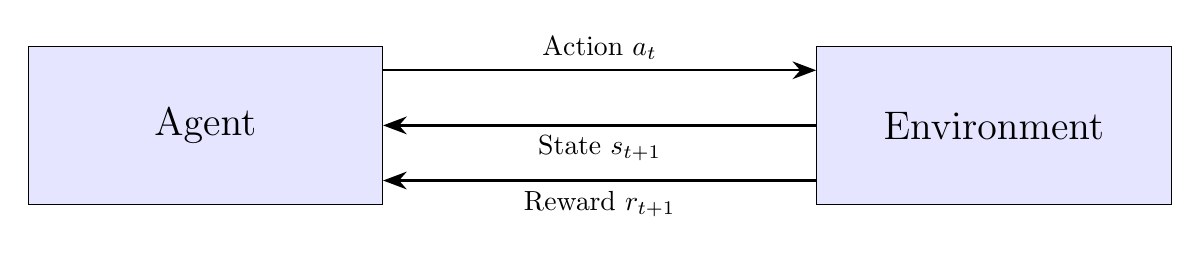
\begin{tikzpicture}[
    node distance=2.5cm,
    block/.style={rectangle, draw, minimum width=4.5cm, minimum height=2cm, align=center, fill=blue!10, font=\Large},
    arrow/.style={-{Stealth[length=3mm]}, thick}
]
    % Agent
    \node[block] (agent) {Agent};

    % Environment
    \node[block, right=5.5cm of agent] (env) {Environment};

    % Arrows - well spaced
    \draw[arrow] ([yshift=0.7cm]agent.east) -- node[above] {Action $a_t$} ([yshift=0.7cm]env.west);
    \draw[arrow] ([yshift=0cm]env.west) -- node[below] {State $s_{t+1}$} ([yshift=0cm]agent.east);
    \draw[arrow] ([yshift=-0.7cm]env.west) -- node[below] {Reward $r_{t+1}$} ([yshift=-0.7cm]agent.east);

\end{tikzpicture}
\caption{Agent-environment interaction in a Markov Decision Process.}
\label{fig:mdp}
\end{figure}

\subsection{Policy and Value Functions}

A policy $\pi$ defines the agent's behavior by specifying which action to take in each state. A deterministic policy $\pi: \mathcal{S} \rightarrow \mathcal{A}$ maps states directly to actions, while a stochastic policy $\pi(a|s)$ represents the probability of selecting action $a$ in state $s$. Stochastic policies enable exploration during learning and arise naturally in multi-agent settings where predictable behavior can be exploited.

The state-value function $V^\pi(s)$ estimates the expected return when starting in state $s$ and following policy $\pi$:
\begin{equation}
V^\pi(s) = \mathbb{E}_\pi\left[\sum_{k=0}^{\infty} \gamma^k R_{t+k+1} \middle| s_t = s\right]
\end{equation}

The action-value function $Q^\pi(s,a)$ estimates the expected return when starting in state $s$, taking action $a$, and following policy $\pi$ thereafter:
\begin{equation}
Q^\pi(s,a) = \mathbb{E}_\pi[G_t | s_t = s, a_t = a]
\end{equation}

The Q-function is particularly useful because it allows action selection without knowing environment dynamics. The optimal policy can be extracted through $\pi^*(s) = \arg\max_{a} Q^*(s,a)$, where $Q^*$ satisfies the Bellman optimality equation:
\begin{equation}
Q^*(s,a) = \sum_{s' \in \mathcal{S}} P(s'|s,a)\left[R(s,a) + \gamma \max_{a'} Q^*(s',a')\right]
\end{equation}

\subsection{Experience Replay and Off-Policy Learning}

A fundamental distinction in reinforcement learning is between on-policy and off-policy methods. On-policy methods (e.g., PPO, A2C) learn from experiences collected by the current policy, offering stability but limited sample efficiency since each experience is used once. Off-policy methods (e.g., DQN) learn from experiences collected by any policy, enabling experience replay, which reuses past transitions multiple times. We experiment with both: DQN uses replay buffers while PPO learns from fresh rollouts.

Experience replay is a critical technique that enables stable training in deep reinforcement learning. The key insight is that training a neural network on consecutive samples from an agent's trajectory creates two problems: (1) consecutive samples are highly correlated, violating the i.i.d. assumption of stochastic gradient descent, and (2) the data distribution shifts as the policy improves, causing catastrophic forgetting of previously learned behaviors.

When training directly on sequential experiences, the network sees a stream of highly correlated transitions. For example, in Snake, consecutive states differ only slightly as the snake moves one cell. This correlation causes the gradient updates to be biased toward recent experiences, leading to oscillating or diverging Q-values. The network effectively ``forgets'' how to handle states it encountered earlier in training.

\begin{figure}[H]
\centering
\begin{subfigure}[b]{0.48\textwidth}
\centering
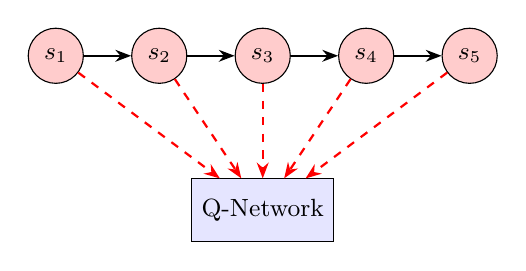
\begin{tikzpicture}[
    node distance=0.6cm,
    state/.style={circle, draw, minimum size=0.7cm, fill=red!20, font=\small},
    arrow/.style={-{Stealth[length=2mm]}, thick},
    dashedarrow/.style={-{Stealth[length=2mm]}, thick, dashed}
]
    % Sequential states
    \node[state] (s1) {$s_1$};
    \node[state, right=of s1] (s2) {$s_2$};
    \node[state, right=of s2] (s3) {$s_3$};
    \node[state, right=of s3] (s4) {$s_4$};
    \node[state, right=of s4] (s5) {$s_5$};

    \draw[arrow] (s1) -- (s2);
    \draw[arrow] (s2) -- (s3);
    \draw[arrow] (s3) -- (s4);
    \draw[arrow] (s4) -- (s5);

    % Neural network
    \node[rectangle, draw, fill=blue!10, minimum width=1.8cm, minimum height=0.8cm, below=1.2cm of s3, font=\small] (nn) {Q-Network};

    % Correlation indicator
    \draw[dashedarrow, red] (s1) -- (nn);
    \draw[dashedarrow, red] (s2) -- (nn);
    \draw[dashedarrow, red] (s3) -- (nn);
    \draw[dashedarrow, red] (s4) -- (nn);
    \draw[dashedarrow, red] (s5) -- (nn);

\end{tikzpicture}
\caption{Without experience replay.}
\label{fig:no_replay}
\end{subfigure}
\hfill
\begin{subfigure}[b]{0.48\textwidth}
\centering
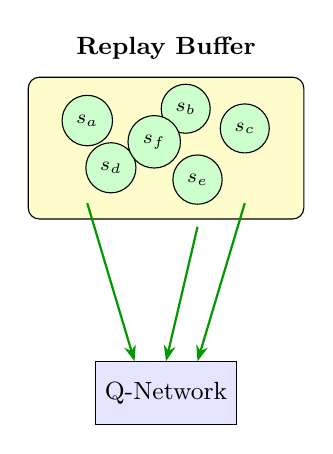
\begin{tikzpicture}[
    node distance=0.5cm,
    state/.style={circle, draw, minimum size=0.5cm, fill=green!20, font=\scriptsize},
    arrow/.style={-{Stealth[length=2mm]}, thick},
    dashedarrow/.style={-{Stealth[length=2mm]}, thick, dashed}
]
    % Replay buffer (cylinder-like)
    \node[rectangle, draw, fill=yellow!20, minimum width=3.5cm, minimum height=1.8cm, rounded corners] (buffer) {};
    \node[above=0.1cm of buffer.north, font=\small\bfseries] {Replay Buffer};

    % States inside buffer (scattered)
    \node[state] at (-1.0, 0.35) {$s_a$};
    \node[state] at (0.25, 0.5) {$s_b$};
    \node[state] at (1.0, 0.25) {$s_c$};
    \node[state] at (-0.7, -0.25) {$s_d$};
    \node[state] at (0.4, -0.4) {$s_e$};
    \node[state] at (-0.15, 0.08) {$s_f$};

    % Neural network
    \node[rectangle, draw, fill=blue!10, minimum width=1.8cm, minimum height=0.8cm, below=1.8cm of buffer, font=\small] (nn) {Q-Network};

    % Random sampling arrows
    \draw[arrow, green!60!black] (-1.0, -0.7) -- ([xshift=-0.4cm]nn.north);
    \draw[arrow, green!60!black] (0.4, -1.0) -- (nn.north);
    \draw[arrow, green!60!black] (1.0, -0.7) -- ([xshift=0.4cm]nn.north);

\end{tikzpicture}
\caption{With experience replay.}
\label{fig:with_replay}
\end{subfigure}
\caption{Experience replay comparison: (a) Sequential training causes correlated updates; (b) Random sampling from a buffer breaks correlations.}
\label{fig:experience_replay}
\end{figure}

Experience replay addresses these issues by storing transitions $(s_t, a_t, r_{t+1}, s_{t+1})$ in a buffer and sampling mini-batches uniformly at random for training. This breaks temporal correlations and provides a more stationary data distribution. The buffer acts as a memory that allows reusing past experiences multiple times, improving sample efficiency.

The replay buffer typically stores the most recent $N$ transitions (e.g., $N = 100,000$), discarding older experiences as new ones arrive. This ensures the buffer contains a diverse set of experiences while remaining bounded in memory.

\subsection{Value-Based Methods}

Value-based methods learn the optimal value function and derive a policy from it. The foundational algorithm in this category is Q-learning \cite{watkins1992q}, which updates Q-values using:
\begin{equation}
Q(s_t, a_t) \leftarrow Q(s_t, a_t) + \alpha \left[R_{t+1} + \gamma \max_{a} Q(s_{t+1}, a) - Q(s_t, a_t)\right]
\end{equation}
where $\alpha$ is the learning rate. The term in brackets is the temporal difference (TD) error, measuring the discrepancy between the current estimate and the bootstrapped target.

For problems with large or continuous state spaces, tabular methods become infeasible. Deep Q-Networks (DQN) address this limitation by using deep neural networks as function approximators for the Q-function \cite{mnih2015human}. DQN introduces two critical innovations that stabilize training. Experience replay stores transitions $(s_t, a_t, r_{t+1}, s_{t+1})$ in a replay buffer and samples mini-batches uniformly for training, breaking temporal correlations and improving sample efficiency. The target network maintains a separate copy of the Q-network with parameters $\theta^-$ that are periodically synchronized with the main network, preventing the instability that arises from chasing a constantly moving target.

The DQN loss function is:
\begin{equation}
L(\theta) = \mathbb{E}_{(s,a,r,s') \sim \mathcal{D}}\left[\left(r + \gamma \max_{a'} Q(s',a';\theta^-) - Q(s,a;\theta)\right)^2\right]
\end{equation}

Several improvements to the basic DQN algorithm have been proposed. Double DQN \cite{van2016deep} addresses the overestimation bias by decoupling action selection from action evaluation, using the online network to select actions and the target network to evaluate them. Dueling DQN \cite{wang2016dueling} separates the Q-function into value and advantage streams: $Q(s,a) = V(s) + A(s,a) - \frac{1}{|\mathcal{A}|}\sum_{a'} A(s,a')$, enabling the network to learn state values independently of action advantages. Prioritized Experience Replay \cite{schaul2016prioritized} samples transitions based on their TD error magnitude, focusing learning on the most informative experiences. Noisy Networks \cite{fortunato2018noisy} replace deterministic layers with noisy ones, providing state-dependent exploration without requiring epsilon-greedy schedules.

\begin{figure}[H]
\centering
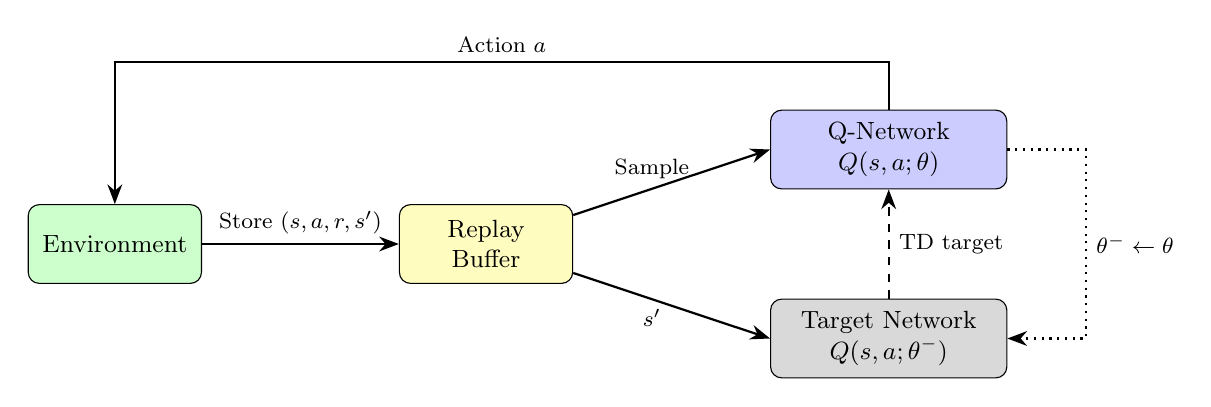
\begin{tikzpicture}[
    node distance=2cm,
    block/.style={rectangle, draw, rounded corners, minimum width=2.2cm, minimum height=1cm, align=center, font=\small},
    netblock/.style={rectangle, draw, rounded corners, minimum width=3cm, minimum height=1cm, align=center, font=\small},
    arrow/.style={-{Stealth[length=2.5mm]}, thick}
]
    % Horizontal layout: Environment -> Replay Buffer -> Networks
    \node[block, fill=green!20] (env) {Environment};
    \node[block, fill=yellow!25, right=2.5cm of env] (buffer) {Replay\\Buffer};

    % Networks stacked vertically on the right (increased spacing, same width)
    \node[netblock, fill=blue!20, right=2.5cm of buffer, yshift=1.2cm] (qnet) {Q-Network\\$Q(s,a;\theta)$};
    \node[netblock, fill=gray!30, right=2.5cm of buffer, yshift=-1.2cm] (target) {Target Network\\$Q(s,a;\theta^-)$};

    % === Main Data Flow ===

    % Environment stores transitions in buffer
    \draw[arrow] (env) -- node[above, font=\footnotesize] {Store $(s,a,r,s')$} (buffer);

    % Buffer feeds both networks
    \draw[arrow] (buffer) -- node[above, font=\footnotesize, pos=0.4] {Sample} (qnet.west);
    \draw[arrow] (buffer) -- node[below, font=\footnotesize, pos=0.4] {$s'$} (target.west);

    % Target provides TD target to Q-network
    \draw[arrow, dashed] (target.north) -- node[right, font=\footnotesize] {TD target} (qnet.south);

    % Q-network outputs action back to environment
    \draw[arrow] (qnet.north) -- ++(0, 0.6) -| node[above, font=\footnotesize, pos=0.25] {Action $a$} (env.north);

    % Periodic weight copy (loops around the right side, ending at target)
    \draw[arrow, dotted, thick] (qnet.east) -- ++(1.0, 0) |- node[right, font=\footnotesize, pos=0.25] {$\theta^- \leftarrow \theta$} (target.east);

\end{tikzpicture}
\caption{DQN training loop.}
\label{fig:dqn}
\end{figure}

Table \ref{tab:dqn_variants} summarizes the DQN variants and their key improvements.

\begin{table}[H]
\centering
\caption{DQN Variants and Improvements}
\label{tab:dqn_variants}
\renewcommand{\arraystretch}{1.5}
\begin{tabular*}{\textwidth}{@{\extracolsep{\fill}}p{1.5cm}p{5cm}p{7cm}@{}}
\toprule
\textbf{Variant} & \textbf{Description} & \textbf{Key Equation} \\
\midrule
DQN & Base algorithm with experience replay and target network & $L(\theta) = \mathbb{E}[(r + \gamma \max_{a'} Q(s',a';\theta^-) - Q(s,a;\theta))^2]$ \\
Double & Decouples action selection from evaluation to reduce overestimation bias & $a^* = \arg\max_a Q(s',a;\theta)$, evaluate with $Q(s',a^*;\theta^-)$ \\
Dueling & Separates Q-function into value and advantage streams & $Q(s,a) = V(s) + A(s,a) - \frac{1}{|\mathcal{A}|}\sum_{a'} A(s,a')$ \\
PER & Samples transitions by TD error magnitude for focused learning & Priority $p_i = |\delta_i| + \epsilon$ \\
Noisy & Adds learnable noise to network weights for exploration & $y = (b + Wz)x$ where $z \sim \mathcal{N}(0,1)$ \\
Rainbow & Combines all improvements: Double, Dueling, PER, Noisy, N-step, Distributional & All of the above + distributional $Q(s,a) \sim \mathcal{Z}$ \\
\bottomrule
\end{tabular*}
\renewcommand{\arraystretch}{1.0}
\end{table}

\subsection{Policy Gradient Methods}

While value-based methods learn a value function and derive a policy from it, policy gradient methods directly parameterize and optimize the policy $\pi_\theta(a|s)$. The objective is to maximize the expected return:
\begin{equation}
J(\theta) = \mathbb{E}_{\tau \sim \pi_\theta}[G(\tau)]
\end{equation}

The policy gradient theorem \cite{williams1992simple} provides a way to compute gradients of this objective:
\begin{equation}
\nabla_\theta J(\theta) = \mathbb{E}_{\tau \sim \pi_\theta}\left[\sum_{t=0}^T \nabla_\theta \log \pi_\theta(a_t|s_t) G_t\right]
\end{equation}

The REINFORCE algorithm uses Monte Carlo estimation of this gradient, updating parameters after each complete episode. To reduce variance, a baseline $b(s_t)$ is subtracted from the return, with the state-value function $V(s_t)$ being a common choice. This leads to the advantage function $A(s,a) = Q(s,a) - V(s)$, which measures how much better an action is compared to the average.

Actor-Critic methods combine value-based and policy-based approaches. The actor (policy network) selects actions while the critic (value network) evaluates them, providing lower-variance gradient estimates. The Advantage Actor-Critic (A2C) algorithm \cite{mnih2016asynchronous} uses the TD error as an estimate of the advantage:
\begin{equation}
A(s_t, a_t) \approx r_{t+1} + \gamma V(s_{t+1}) - V(s_t)
\end{equation}

Proximal Policy Optimization (PPO) \cite{schulman2017proximal} has become one of the most popular RL algorithms due to its simplicity and effectiveness. Building on Trust Region Policy Optimization (TRPO) \cite{schulman2015trust}, PPO constrains policy updates to prevent large, destabilizing changes using a clipped surrogate objective:
\begin{equation}
L^{CLIP}(\theta) = \mathbb{E}_t\left[\min\left(r_t(\theta)A_t, \text{clip}(r_t(\theta), 1-\epsilon, 1+\epsilon)A_t\right)\right]
\end{equation}
where $r_t(\theta) = \frac{\pi_\theta(a_t|s_t)}{\pi_{\theta_{old}}(a_t|s_t)}$ is the probability ratio. The clipping prevents the policy from changing too drastically in a single update. PPO also uses Generalized Advantage Estimation (GAE) \cite{schulman2016high} to balance bias and variance in advantage estimates:
\begin{equation}
A_t^{GAE} = \sum_{l=0}^{\infty} (\gamma\lambda)^l \delta_{t+l}
\end{equation}
where $\delta_t = r_t + \gamma V(s_{t+1}) - V(s_t)$ is the TD error and $\lambda$ controls the trade-off.

\begin{figure}[H]
\centering
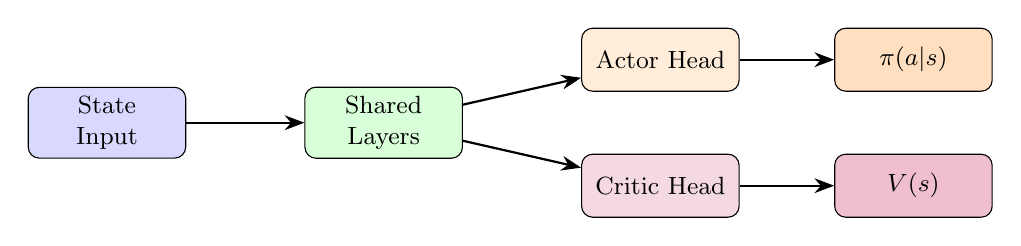
\begin{tikzpicture}[
    node distance=1.5cm,
    block/.style={rectangle, draw, rounded corners, minimum width=2cm, minimum height=0.8cm, align=center, font=\small},
    arrow/.style={-{Stealth[length=2.5mm]}, thick}
]
    % Horizontal layout: Input -> Shared -> Actor/Critic branches
    \node[block, fill=blue!15] (input) {State\\Input};
    \node[block, fill=green!15, right=1.5cm of input] (shared) {Shared\\Layers};

    % Actor branch (top)
    \node[block, fill=orange!15, right=1.5cm of shared, yshift=0.8cm] (actor) {Actor Head};
    \node[block, fill=orange!25, right=1.2cm of actor] (policy) {$\pi(a|s)$};

    % Critic branch (bottom)
    \node[block, fill=purple!15, right=1.5cm of shared, yshift=-0.8cm] (critic) {Critic Head};
    \node[block, fill=purple!25, right=1.2cm of critic] (value) {$V(s)$};

    % Arrows
    \draw[arrow] (input) -- (shared);
    \draw[arrow] (shared) -- (actor);
    \draw[arrow] (shared) -- (critic);
    \draw[arrow] (actor) -- (policy);
    \draw[arrow] (critic) -- (value);

\end{tikzpicture}
\caption{Actor-Critic architecture.}
\label{fig:actor_critic}
\end{figure}

Table \ref{tab:policy_gradient_methods} summarizes the policy gradient methods we consider.

\begin{table}[H]
\centering
\caption{Policy Gradient Methods Comparison}
\label{tab:policy_gradient_methods}
\renewcommand{\arraystretch}{1.5}
\begin{tabular*}{\textwidth}{@{\extracolsep{\fill}}p{2cm}p{4.5cm}p{7cm}@{}}
\toprule
\textbf{Method} & \textbf{Description} & \textbf{Key Equation} \\
\midrule
REINFORCE & Monte Carlo policy gradient with episode returns & $\nabla J = \mathbb{E}[\sum_t \nabla \log \pi(a_t|s_t) G_t]$ \\
A2C & Advantage Actor-Critic with TD advantage estimation & $A(s_t,a_t) = r_{t+1} + \gamma V(s_{t+1}) - V(s_t)$ \\
PPO & Clipped surrogate objective for stable updates & $L = \min(r_t A_t, \text{clip}(r_t, 1\pm\epsilon) A_t)$ \\
\bottomrule
\end{tabular*}
\renewcommand{\arraystretch}{1.0}
\end{table}

%==============================================================================
% SECTION 3: IMPLEMENTATION
%==============================================================================
\section{Implementation}

This section describes our implementation of the Snake game environments and reinforcement learning infrastructure. We detail the environment design, state representations, network architectures, and training procedures.

\subsection{Code Structure}

Our implementation follows a modular architecture organized into several components. The \texttt{core/} directory contains core modules including environments, neural networks, state representations, and utilities. Training scripts for each algorithm (DQN, PPO, A2C) reside in \texttt{scripts/training/}, while \texttt{scripts/visualizer/} provides visualization and recording tools. The \texttt{results/} directory stores trained weights, training data, and generated figures.

All environments follow the Gymnasium (OpenAI Gym) API standard, ensuring compatibility with standard RL libraries. The environment features a configurable grid (default $10 \times 10$) where the snake starts with length 3 at the center. Food appears randomly on empty cells, and episodes terminate upon collision with walls or the snake's body, or after a timeout of $2 \times \text{grid\_area}$ steps without collecting food.

\subsection{Environment Design}

The action space uses relative directions rather than absolute directions. STRAIGHT (0) continues in the current direction, RIGHT\_TURN (1) turns 90 degrees clockwise, and LEFT\_TURN (2) turns 90 degrees counter-clockwise. This relative action space offers several advantages over absolute directions (UP, DOWN, LEFT, RIGHT): the action space is reduced from 4 to 3 actions simplifying the learning problem, 180-degree turns (instant death) are impossible by construction, and the agent learns behaviors that generalize across all orientations. The relative encoding means the agent's decision depends only on what lies ahead, to the right, and to the left, not on absolute compass directions. This invariance reduces the effective state space the agent must learn.

\begin{figure}[H]
\centering
\begin{subfigure}[b]{0.45\textwidth}
\centering
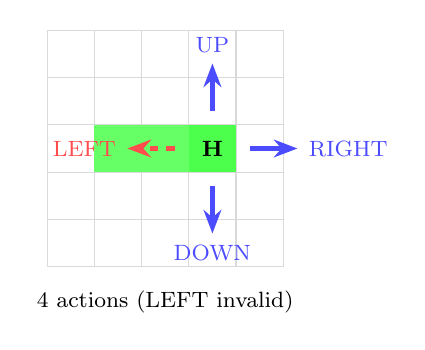
\begin{tikzpicture}[scale=0.6]
    % Grid
    \draw[step=1, gray!30, thin] (0,0) grid (5,5);

    % Snake body (going right)
    \fill[green!60] (1,2) rectangle (2,3);
    \fill[green!60] (2,2) rectangle (3,3);
    \fill[green!70] (3,2) rectangle (4,3);  % Head

    % Head marker
    \node at (3.5,2.5) {\footnotesize\textbf{H}};

    % Absolute direction arrows
    \draw[-{Stealth[length=3mm]}, ultra thick, blue!70] (3.5,3.3) -- (3.5,4.3) node[above] {\footnotesize UP};
    \draw[-{Stealth[length=3mm]}, ultra thick, blue!70] (3.5,1.7) -- (3.5,0.7) node[below] {\footnotesize DOWN};
    \draw[-{Stealth[length=3mm]}, ultra thick, blue!70] (4.3,2.5) -- (5.3,2.5) node[right] {\footnotesize RIGHT};
    \draw[-{Stealth[length=3mm]}, ultra thick, red!70, dashed] (2.7,2.5) -- (1.7,2.5) node[left] {\footnotesize LEFT};

    % Note
    \node[below] at (2.5,-0.3) {\footnotesize 4 actions (LEFT invalid)};
\end{tikzpicture}
\caption{Absolute directions}
\label{fig:absolute_dir}
\end{subfigure}
\hfill
\begin{subfigure}[b]{0.45\textwidth}
\centering
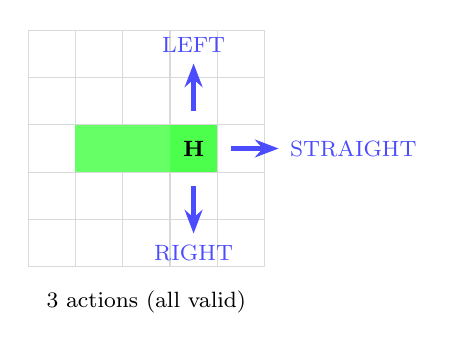
\begin{tikzpicture}[scale=0.6]
    % Grid
    \draw[step=1, gray!30, thin] (0,0) grid (5,5);

    % Snake body (going right)
    \fill[green!60] (1,2) rectangle (2,3);
    \fill[green!60] (2,2) rectangle (3,3);
    \fill[green!70] (3,2) rectangle (4,3);  % Head

    % Head marker
    \node at (3.5,2.5) {\footnotesize\textbf{H}};

    % Relative direction arrows
    \draw[-{Stealth[length=3mm]}, ultra thick, blue!70] (4.3,2.5) -- (5.3,2.5) node[right] {\footnotesize STRAIGHT};
    \draw[-{Stealth[length=3mm]}, ultra thick, blue!70] (3.5,1.7) -- (3.5,0.7) node[below] {\footnotesize RIGHT};
    \draw[-{Stealth[length=3mm]}, ultra thick, blue!70] (3.5,3.3) -- (3.5,4.3) node[above] {\footnotesize LEFT};

    % Note
    \node[below] at (2.5,-0.3) {\footnotesize 3 actions (all valid)};
\end{tikzpicture}
\caption{Relative directions}
\label{fig:relative_dir}
\end{subfigure}
\caption{Action space comparison.}
\label{fig:action_space}
\end{figure}

The reward function guides learning behavior through immediate feedback signals. Table~\ref{tab:rewards} summarizes the reward structure.

\begin{table}[H]
\centering
\caption{Reward Function}
\label{tab:rewards}
\begin{tabular}{lrl}
\toprule
\textbf{Event} & \textbf{Reward} & \textbf{Purpose} \\
\midrule
Food consumption & +10 & Primary objective \\
Collision/death & $-10$ & Survival penalty \\
Time step & $-0.01$ & Efficiency incentive \\
Move toward food & +1 & Reward shaping (optional) \\
Move away from food & $-1$ & Reward shaping (optional) \\
\bottomrule
\end{tabular}
\end{table}

The time penalty provides dense feedback encouraging efficient food collection rather than aimless wandering. Distance-based shaping accelerates early learning but is optional.

\subsection{State Representations}

State representation significantly impacts learning efficiency and final performance. We designed two representations with increasing sophistication: a basic 10-dimensional feature vector and a 13-dimensional representation with flood-fill features.

The simplest representation uses 10 dimensions capturing immediate spatial awareness. This includes three binary danger indicators for collision risk in relative directions (straight, right, left), four binary food direction indicators showing whether food lies up, right, down, or left relative to the head, and three one-hot encoded features representing the snake's current relative direction. This basic representation provides sufficient information for learning fundamental navigation skills.

Building on this foundation, we developed a 13-dimensional representation that adds flood-fill features. These three additional features measure the ratio of reachable cells in each relative direction using a breadth-first traversal similar to BFS. By computing how much free space is accessible from potential next positions, the agent can avoid moves leading to dead-ends or self-trapping situations. The flood-fill computation normalizes values by the maximum possible free cells, producing features in the range [0, 1].

For CNN-based approaches, we use a grid representation with 3 channels encoding head position, body position, and food position respectively. This raw grid input requires convolutional layers to extract spatial features but provides complete spatial information without hand-crafted feature engineering.

\begin{figure}[H]
\centering
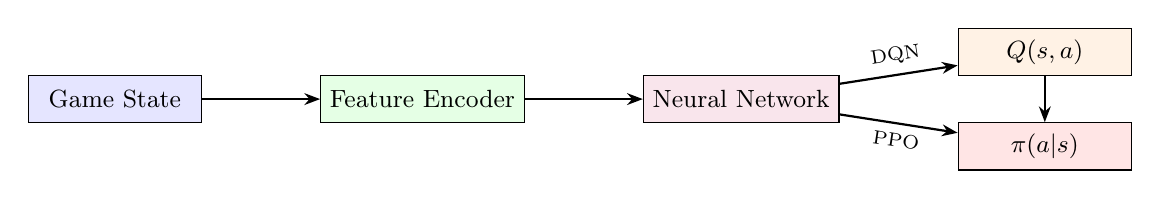
\begin{tikzpicture}[
    node distance=1cm,
    box/.style={rectangle, draw, minimum width=2.2cm, minimum height=0.6cm, align=center, font=\small},
    arrow/.style={-{Stealth[length=2mm]}, thick}
]
    % Horizontal flow: Game State -> Feature Encoder -> Neural Network -> Output
    \node[box, fill=blue!10] (state) {Game State};
    \node[box, fill=green!10, right=1.5cm of state] (encoder) {Feature Encoder};
    \node[box, fill=purple!10, right=1.5cm of encoder] (network) {Neural Network};

    % Q-value box (for DQN path)
    \node[box, fill=orange!10, right=1.5cm of network, yshift=0.6cm] (qvalue) {$Q(s,a)$};

    % Policy box (final output for both)
    \node[box, fill=red!10, right=1.5cm of network, yshift=-0.6cm] (policy) {$\pi(a|s)$};

    % Common path
    \draw[arrow] (state) -- (encoder);
    \draw[arrow] (encoder) -- (network);

    % DQN path: NN -> Q -> pi (labeled)
    \draw[arrow] (network) -- node[above, font=\scriptsize, sloped] {DQN} (qvalue);
    \draw[arrow] (qvalue) -- (policy);

    % PPO path: NN -> pi directly (labeled)
    \draw[arrow] (network) -- node[below, font=\scriptsize, sloped] {PPO} (policy);

\end{tikzpicture}
\caption{State representation pipeline.}
\label{fig:state_rep}
\end{figure}

\subsection{Network Architectures}

We implement two network architectures: MLP for feature-based inputs and CNN for grid-based inputs.

For MLP-based agents with feature input, we use two hidden layers with 128 neurons each and ReLU activations. The output layer produces Q-values (for DQN) or action logits (for policy gradient methods). For CNN-based agents with grid input, we use three convolutional layers (32, 64, 64 filters with 3x3 kernels), followed by a fully connected layer (256 neurons) and the output layer. Padding preserves spatial dimensions through the convolutional layers.

\begin{figure}[H]
\centering
\begin{subfigure}[c]{0.45\textwidth}
\centering
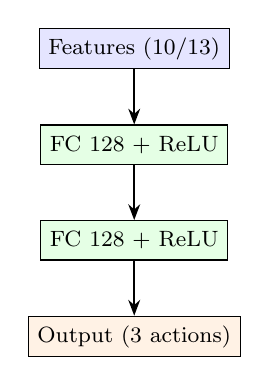
\begin{tikzpicture}[
    node distance=0.7cm,
    layer/.style={rectangle, draw, minimum width=2.2cm, minimum height=0.5cm, align=center, font=\footnotesize},
    arrow/.style={-{Stealth[length=2mm]}, thick}
]
    \node[layer, fill=blue!10] (input) {Features (10/13)};
    \node[layer, fill=green!10, below=of input] (fc1) {FC 128 + ReLU};
    \node[layer, fill=green!10, below=of fc1] (fc2) {FC 128 + ReLU};
    \node[layer, fill=orange!10, below=of fc2] (output) {Output (3 actions)};

    \draw[arrow] (input) -- (fc1);
    \draw[arrow] (fc1) -- (fc2);
    \draw[arrow] (fc2) -- (output);
\end{tikzpicture}
\caption{MLP for feature-based input.}
\label{fig:mlp_arch}
\end{subfigure}
\hfill
\begin{subfigure}[c]{0.45\textwidth}
\centering
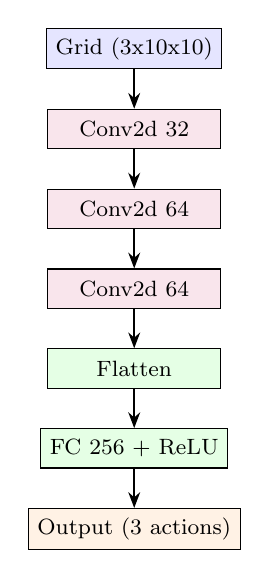
\begin{tikzpicture}[
    node distance=0.5cm,
    layer/.style={rectangle, draw, minimum width=2.2cm, minimum height=0.5cm, align=center, font=\footnotesize},
    arrow/.style={-{Stealth[length=2mm]}, thick}
]
    \node[layer, fill=blue!10] (input) {Grid (3x10x10)};
    \node[layer, fill=purple!10, below=of input] (conv1) {Conv2d 32};
    \node[layer, fill=purple!10, below=of conv1] (conv2) {Conv2d 64};
    \node[layer, fill=purple!10, below=of conv2] (conv3) {Conv2d 64};
    \node[layer, fill=green!10, below=of conv3] (flatten) {Flatten};
    \node[layer, fill=green!10, below=of flatten] (fc) {FC 256 + ReLU};
    \node[layer, fill=orange!10, below=of fc] (output) {Output (3 actions)};

    \draw[arrow] (input) -- (conv1);
    \draw[arrow] (conv1) -- (conv2);
    \draw[arrow] (conv2) -- (conv3);
    \draw[arrow] (conv3) -- (flatten);
    \draw[arrow] (flatten) -- (fc);
    \draw[arrow] (fc) -- (output);
\end{tikzpicture}
\caption{CNN for grid-based input.}
\label{fig:cnn_arch}
\end{subfigure}
\caption{Network architectures.}
\label{fig:network_archs}
\end{figure}

Although CNNs are well-suited for spatial feature detection and could theoretically scale better to larger grid sizes by leveraging GPU parallelism for convolution operations, in practice CNNs are slower to run than MLPs with hand-crafted features. The convolutional operations add computational overhead that outweighs their benefits for our relatively small $10 \times 10$ grid. For this problem size, the MLP with flood-fill features provides both better performance and faster inference.

PPO uses separate actor and critic networks, or a shared backbone with separate heads. The actor outputs action logits processed through softmax for action probabilities. The critic outputs a single scalar value estimate.

\subsection{Vectorized Environment Training}

A key contribution of our implementation is vectorized environments using PyTorch tensors. Instead of running a single game sequentially, we run 128-256 simultaneous games in parallel. All game state (snake positions, food locations, directions) is stored as batched tensors, and game logic (collision detection, movement, reward computation) is implemented using vectorized tensor operations.

This vectorization enables a 40$\times$ speedup compared to sequential single-environment training by amortizing Python interpreter overhead. With 256 parallel environments on CPU, DQN achieves $\sim$4,800 episodes per minute compared to only $\sim$120 episodes/min with a single environment. For algorithms with higher computational cost per step (PPO with flood-fill features), speedups are more modest but still substantial at $\sim$4$\times$. Notably, for single-snake training with small neural networks (2-3 hidden layers, 128--256 units), all computation runs on CPU; GPU acceleration provides no benefit because the neural network operations are too small to overcome memory transfer overhead. The key speedup comes entirely from environment parallelization. Training 3,000 DQN episodes with basic features completes in under 1 minute, while 3,000 PPO episodes with flood-fill features takes approximately 27 minutes.

\subsection{Training Procedures}

We implemented training scripts for all algorithms with consistent interfaces and configurable hyperparameters. Table \ref{tab:hyperparameters} summarizes key hyperparameters.

\begin{table}[H]
\centering
\caption{Training Hyperparameters}
\label{tab:hyperparameters}
\begin{tabular}{lcc}
\toprule
\textbf{Parameter} & \textbf{DQN} & \textbf{PPO} \\
\midrule
Learning rate & 0.001 & 0.0003 \\
Discount factor ($\gamma$) & 0.99 & 0.99 \\
Batch size & 64 & 64 \\
Buffer/Rollout size & 100,000 & 2,048 \\
Hidden layers & 128x128 & 128x128 \\
$\epsilon$ start/end & 1.0/0.01 & N/A \\
$\epsilon$ decay & 0.995 & N/A \\
Clip parameter & N/A & 0.2 \\
GAE $\lambda$ & N/A & 0.95 \\
Entropy coefficient & N/A & 0.01 \\
Target update freq & 1,000 steps & N/A \\
\bottomrule
\end{tabular}
\end{table}

For DQN variants, we train for 3,000 episodes with 256 parallel environments. Training uses Adam optimizer with gradient clipping (max norm 1.0). The replay buffer stores transitions and samples uniformly (or by priority for PER). The target network updates every 1,000 training steps.

For policy gradient methods, we collect rollouts of 2,048 steps across parallel environments, then perform multiple epochs (4-10) of mini-batch updates. PPO uses the clipped objective with value function and entropy bonuses. A2C uses simpler advantage estimation without clipping.

%==============================================================================
% SECTION 4: EXPERIMENTS
%==============================================================================
\section{Experiments}

This section presents our experimental results, organized to demonstrate the progression of our investigation. We begin with vanilla implementations of DQN and PPO, then explore DQN variants. We investigate death causes to understand failure modes, first attempt reward system modifications, then introduce flood-fill features as the comprehensive solution. We demonstrate grid size generalization and finally present results from the competitive two-snake environment. Appendix~\ref{app:algorithm_comparison} provides comprehensive results for all nine algorithms.

\subsection{Vanilla DQN and PPO}

We first establish baseline performance with standard implementations of DQN and PPO using basic features (danger indicators, food direction, current direction). Both algorithms were trained with 256 parallel environments on a $10 \times 10$ grid. DQN was trained for 3,000 episodes, while PPO achieved comparable results in 2,000 episodes due to its superior sample efficiency.

\textbf{Figure \ref{fig:dqn_results}} shows DQN training progression with basic features, demonstrating the characteristic learning curve with initial exploration phase followed by exploitation. \textbf{Figure \ref{fig:ppo_results}} shows PPO training, which exhibits faster convergence and more stable learning dynamics.

\begin{figure}[H]
\centering
\begin{subfigure}[b]{0.48\textwidth}
\centering
\includegraphics[width=\textwidth]{dqn_basic_scores.png}
\caption{DQN training curve.}
\label{fig:dqn_results}
\end{subfigure}
\hfill
\begin{subfigure}[b]{0.48\textwidth}
\centering
\includegraphics[width=\textwidth]{ppo_basic_scores.png}
\caption{PPO training curve.}
\label{fig:ppo_results}
\end{subfigure}
\caption{Training with basic features.}
\label{fig:basic_training}
\end{figure}

PPO consistently outperforms DQN in sample efficiency, achieving comparable or better final scores in fewer episodes. This advantage stems from PPO's on-policy learning with entropy regularization, which maintains exploration throughout training, unlike DQN's decaying epsilon-greedy strategy.

\subsection{DQN Variants}

We evaluated several DQN improvements to understand their individual contributions. Double DQN reduces overestimation bias by decoupling action selection from evaluation. Dueling DQN separates value and advantage streams for better state evaluation. Prioritized Experience Replay (PER) focuses learning on high-error transitions. Noisy Networks replaces epsilon-greedy with learnable exploration.

In our experiments, Double DQN provided the most consistent improvement, reducing Q-value overestimation that can destabilize learning. Dueling DQN showed benefits in states where most actions have similar value. PER accelerated early learning but required careful tuning of priority parameters. Noisy networks eliminated the need for epsilon scheduling but required longer training to learn appropriate exploration levels.

Rainbow DQN \cite{hessel2018rainbow} combines multiple DQN improvements into a single agent: Double Q-learning for reduced overestimation, Dueling architecture for better value estimation, Prioritized Experience Replay for efficient sampling, Noisy networks for exploration, and Distributional RL for modeling return distributions. Our implementation uses 51 atoms with support range [-20, 500] to capture the full reward distribution. In our experiments with basic features, Rainbow DQN achieves an average score of 17.94 $\pm$ 6.59, comparable to other DQN variants. The combination of improvements provides stability but does not dramatically outperform simpler variants in our Snake environment, likely because the relatively simple state space does not fully leverage Rainbow's distributional modeling capabilities.

\subsection{Death Cause Analysis}

Understanding why agents die provides insight into failure modes. We categorize deaths into three types: wall collisions (hitting the grid boundary), self-collisions (hitting the snake's own body during normal movement), and entrapments (the snake boxes itself in with no valid escape moves).

\textbf{Figures \ref{fig:dqn_deaths}} and \textbf{\ref{fig:ppo_deaths}} show cumulative death causes over training episodes with basic features.

\begin{figure}[H]
\centering
\begin{subfigure}[b]{0.48\textwidth}
\centering
\includegraphics[width=\textwidth]{dqn_basic_deaths.png}
\caption{DQN death causes.}
\label{fig:dqn_deaths}
\end{subfigure}
\hfill
\begin{subfigure}[b]{0.48\textwidth}
\centering
\includegraphics[width=\textwidth]{ppo_basic_deaths.png}
\caption{PPO death causes.}
\label{fig:ppo_deaths}
\end{subfigure}
\caption{Death causes with basic features.}
\label{fig:basic_deaths}
\end{figure}

With basic features, entrapment is the dominant death cause at 67-86\% of deaths, indicating that agents without spatial awareness frequently maneuver into positions from which escape is impossible. Notably, PPO's wall and self-collision curves flatten toward the end of training, indicating the agent has essentially learned to avoid these immediate dangers completely, yet it still dies frequently from entrapment, which requires longer-term spatial planning.

\subsection{Reward System Modification}

Before investigating feature engineering, we first explored whether reward design could reduce deaths. Specifically, we studied the death penalty hyperparameter with basic features, testing values from -10 to -100. This parameter controls how strongly the agent is penalized for dying, potentially affecting the exploration-exploitation trade-off and learned risk tolerance.

Table \ref{tab:ppo_penalty_basic} shows PPO results across death penalties with basic features. The penalty has moderate impact, with all values producing similar average scores in the 18-20 range. The best performance (-100 penalty) achieves 19.93 average, only marginally better than the baseline -10 penalty (19.48).

\begin{table}[H]
\centering
\caption{PPO Death Penalty Study with Basic Features}
\label{tab:ppo_penalty_basic}
\begin{tabular}{ccc}
\toprule
\textbf{Death Penalty} & \textbf{Avg Score} & \textbf{Max Score} \\
\midrule
-10 & 19.48 & \textbf{45} \\
-20 & 18.40 & \textbf{45} \\
-30 & 18.25 & 40 \\
-40 & 19.30 & 41 \\
-50 & 19.25 & 40 \\
-100 & \textbf{19.93} & 39 \\
\bottomrule
\end{tabular}
\end{table}

The limited impact of reward tuning on performance suggests that the fundamental limitation lies in state representation, not reward design. The agent cannot avoid entrapment regardless of how heavily death is penalized because it lacks the spatial awareness to perceive dead-ends. This motivates the flood-fill feature engineering described in the next section.

\subsection{Flood-Fill Feature Engineering}

The flood-fill feature gives the agent spatial awareness about reachable free space. For each potential next position, we compute the ratio of cells reachable via breadth-first flood-fill traversal (see Algorithm~\ref{alg:floodfill} in Appendix~\ref{app:floodfill}). The result is a value in [0, 1] representing the fraction of free space reachable from that direction. Low values indicate potential dead-ends; high values indicate open space.

\textbf{Figures \ref{fig:dqn_flood}} and \textbf{\ref{fig:ppo_flood}} demonstrate the dramatic improvement in training scores from flood-fill features compared to the basic feature results shown in \textbf{Figures \ref{fig:dqn_results}} and \textbf{\ref{fig:ppo_results}}.

\begin{figure}[H]
\centering
\begin{subfigure}[b]{0.48\textwidth}
\centering
\includegraphics[width=\textwidth]{dqn_flood-fill_scores.png}
\caption{DQN training curve.}
\label{fig:dqn_flood}
\end{subfigure}
\hfill
\begin{subfigure}[b]{0.48\textwidth}
\centering
\includegraphics[width=\textwidth]{ppo_flood-fill_scores.png}
\caption{PPO training curve.}
\label{fig:ppo_flood}
\end{subfigure}
\caption{Training with flood-fill features.}
\label{fig:flood_training}
\end{figure}

Table \ref{tab:representation_comparison} compares performance with and without flood-fill features. The flood-fill representation improves average scores by 52\% for DQN and 99\% for PPO, representing the single most impactful improvement in our experiments.

\begin{table}[H]
\centering
\caption{Single-Snake Performance: Basic vs Flood-fill Features}
\label{tab:representation_comparison}
\begin{tabular}{llcccc}
\toprule
\textbf{Algorithm} & \textbf{Features} & \textbf{Avg Score} & \textbf{Std} & \textbf{Max} & \textbf{Entrap \%} \\
\midrule
DQN & Basic & 16.78 & 6.91 & 43 & 67\% \\
DQN & Flood-fill & 25.44 & 10.98 & 51 & 45\% \\
PPO & Basic & 17.69 & 5.80 & 43 & 86\% \\
PPO & Flood-fill & 35.27 & 6.65 & 58 & 49\% \\
\bottomrule
\end{tabular}
\end{table}

With flood-fill, entrapment drops from 67-86\% to 45-49\% of deaths, explaining the doubled scores. \textbf{Figures \ref{fig:dqn_flood_deaths}} and \textbf{\ref{fig:ppo_flood_deaths}} show this improvement.

\begin{figure}[H]
\centering
\begin{subfigure}[b]{0.48\textwidth}
\centering
\includegraphics[width=\textwidth]{dqn_flood-fill_deaths.png}
\caption{DQN death causes.}
\label{fig:dqn_flood_deaths}
\end{subfigure}
\hfill
\begin{subfigure}[b]{0.48\textwidth}
\centering
\includegraphics[width=\textwidth]{ppo_flood-fill_deaths.png}
\caption{PPO death causes.}
\label{fig:ppo_flood_deaths}
\end{subfigure}
\caption{Death causes with flood-fill features.}
\label{fig:flood_deaths}
\end{figure}

An unexpected observation from the flood-fill experiments is the reintroduction of wall and self-collision deaths. With basic features, entrapment dominated (67-86\% of deaths), but with flood-fill, wall and self-collisions become more prominent again. This suggests that while flood-fill successfully addresses spatial awareness for avoiding dead-ends, the agent may become overconfident in tight spaces or take riskier paths.

We also investigated whether reward tuning could further improve flood-fill performance. Table \ref{tab:ppo_penalty_flood} shows PPO results across death penalties with flood-fill features. The -100 penalty produces the best average score of 39.74, a modest improvement over the baseline -10 penalty (35.08). Combined with our earlier basic feature results (Table \ref{tab:ppo_penalty_basic}), this confirms that state representation has a larger impact than reward tuning: switching from basic to flood-fill features provides an 18-point improvement, while penalty tuning yields at most 4-5 points.

\begin{table}[H]
\centering
\caption{PPO Death Penalty Study with Flood-fill Features}
\label{tab:ppo_penalty_flood}
\begin{tabular}{ccc}
\toprule
\textbf{Death Penalty} & \textbf{Avg Score} & \textbf{Max Score} \\
\midrule
-10 & 35.27 & 58 \\
-20 & 35.91 & 60 \\
-30 & 36.98 & \textbf{64} \\
-40 & 37.52 & 59 \\
-50 & 36.76 & 58 \\
-100 & \textbf{39.74} & 56 \\
\bottomrule
\end{tabular}
\end{table}

\subsection{Grid Size Generalization}

A key advantage of our feature-based state representation is grid-size independence. Because the features encode relative spatial information (danger indicators, food direction, flood-fill ratios) rather than absolute positions, an agent trained on a $10 \times 10$ grid can generalize to larger or smaller grids without retraining.

To validate this, we trained a DQN agent with flood-fill features on a $10 \times 10$ grid for 3,000 episodes, then evaluated its performance on $8 \times 8$, $10 \times 10$, $15 \times 15$, and $20 \times 20$ grids without any additional training. Table \ref{tab:grid_generalization} summarizes the results.

\begin{table}[H]
\centering
\caption{Grid Size Generalization: Model Trained on 10x10, Evaluated on Multiple Sizes}
\label{tab:grid_generalization}
\begin{tabular}{lcccc}
\toprule
\textbf{Grid Size} & \textbf{Avg Score} & \textbf{Max Score} & \textbf{Theoretical Max} & \textbf{\% of Max} \\
\midrule
$8 \times 8$ & 20.0 & 34 & 61 & 32.8\% \\
$10 \times 10$ (trained) & 26.4 & 42 & 97 & 27.2\% \\
$15 \times 15$ & 45.1 & 68 & 222 & 20.3\% \\
$20 \times 20$ & 52.3 & 64 & 397 & 13.2\% \\
\bottomrule
\end{tabular}
\end{table}

The results demonstrate successful generalization across grid sizes. Absolute scores actually increase on larger grids because the snake has more room to maneuver before facing space constraints. The percentage of theoretical maximum decreases for larger grids, which is expected since filling a larger grid requires longer survival and more strategic planning.

\begin{figure}[H]
\centering
\includegraphics[width=0.95\textwidth]{grid_size_generalization.png}
\caption{Grid size generalization.}
\label{fig:grid_generalization}
\end{figure}

The feature encoder only requires normalizing flood-fill values by the new grid's maximum free cells. All other features (danger indicators, food direction, current direction) remain unchanged, enabling zero-shot transfer to unseen grid sizes.

\subsection{Two-Snake Competitive Environment}

Competitive training proved more challenging than single-snake scenarios, requiring curriculum learning for stable performance. In the two-snake environment, both agents share the grid and compete for food, introducing non-stationarity as each agent's policy evolves during training. A round ends when one snake reaches the target food count (10) or when a snake dies.

For competitive scenarios, we designed a 33-dimensional state representation with three feature groups: self-awareness (13 dims) including danger indicators, food direction, current direction, and flood-fill; opponent-awareness (14 dims) including opponent position, direction, length, distance, and threat level; and competitive metrics (6 dims) including length difference, food advantage, and space control. The reward function uses food consumption (+10), death (-50 to -100), winning (+100), and opponent death (+50).

We investigate whether larger networks produce better competitive agents by training two agents with different network capacities: a Big network with 256x256 hidden layers (131,000+ parameters) and a Small network with 128x128 hidden layers (33,000+ parameters). The hypothesis is that competitive scenarios require more representational capacity to model opponent behavior, strategic planning, and multi-objective optimization (food collection vs. survival vs. blocking opponent).

Competitive multi-agent RL introduces several challenges absent in single-agent settings \cite{lowe2017multi}. Non-stationarity arises because the opponent's policy changes during training, violating the stationarity assumption of most RL algorithms. Credit assignment becomes difficult: when one snake dies, it is unclear whether this resulted from its own mistake or the opponent's skill. Reward design must balance food collection, survival, and competitive objectives. Finally, exploration collapse can occur when both agents converge to avoiding each other rather than competing.

Unlike single-snake training where GPU acceleration provides no benefit, competitive two-snake training benefits significantly from GPU computation. Training two neural networks simultaneously with larger PPO rollout batches creates sufficient computational load to overcome GPU memory transfer overhead. Our benchmarks show PPO two-snake training achieves 4.8$\times$ speedup on GPU (1,615 steps/second) compared to CPU (333 steps/second). DQN shows no GPU benefit even in two-snake scenarios due to its smaller batch sizes from experience replay sampling.

Our initial approach was direct co-evolution: training both agents simultaneously from random initialization. This approach failed to produce capable agents. Both snakes learned to avoid the center of the grid and each other, resulting in passive play with neither agent collecting food efficiently.

The failure occurs because early in training, random policies cause frequent collisions. The agents learn that approaching the opponent is dangerous, but this learned avoidance prevents them from developing competitive food-collection strategies. \textbf{Figure \ref{fig:curriculum_stages_both}} shows the curriculum progression through stages 0-3 for both network sizes.

\begin{figure}[H]
\centering
\begin{subfigure}[b]{0.48\textwidth}
\centering
\includegraphics[width=\textwidth]{curriculum_128x128_stages.png}
\caption{128x128 network.}
\label{fig:curriculum_128}
\end{subfigure}
\hfill
\begin{subfigure}[b]{0.48\textwidth}
\centering
\includegraphics[width=\textwidth]{curriculum_256x256_stages.png}
\caption{256x256 network.}
\label{fig:curriculum_256}
\end{subfigure}
\caption{Curriculum learning progression.}
\label{fig:curriculum_stages_both}
\end{figure}

To address co-evolution failure, we employ a five-stage curriculum with progressively increasing opponent difficulty. Stages 0-3 train each network independently against scripted opponents, while Stage 4 pits the 128x128 and 256x256 networks against each other in co-evolution. Table \ref{tab:curriculum_stages} summarizes the curriculum design. Each stage requires achieving both the minimum training steps and the win rate threshold before advancing. The max-steps safety limit ensures progress even if the threshold proves too difficult.

\begin{table}[H]
\centering
\caption{Curriculum Learning Design: 5-Stage Progressive Training}
\label{tab:curriculum_stages}
\begin{tabular}{clcccc}
\toprule
\textbf{Stage} & \textbf{Opponent} & \textbf{Min Steps} & \textbf{Max Steps} & \textbf{Threshold} & \textbf{Target Food} \\
\midrule
0 & Static & 0.5M & 1M & 95\% & 10 \\
1 & Random & 0.5M & 1M & 95\% & 10 \\
2 & Greedy & 3M & 6M & 35\% & 4 \\
3 & Frozen (self) & 2M & 4M & 90\% & 6 \\
4 & Co-evolution & 14M & 14M & --- & 8 \\
\bottomrule
\end{tabular}
\end{table}

The frozen opponent in Stage 3 is a snapshot of the agent's own policy from the end of Stage 2. This self-play stage helps the agent develop strategies against policies similar to its own before facing a live, adapting opponent in co-evolution.

\begin{figure}[H]
\centering
\begin{subfigure}[b]{0.48\textwidth}
\centering
\includegraphics[width=\textwidth]{ppo_direct_coevolution_14M.png}
\caption{Direct co-evolution.}
\label{fig:ppo_direct_coevo}
\end{subfigure}
\hfill
\begin{subfigure}[b]{0.48\textwidth}
\centering
\includegraphics[width=\textwidth]{coevolution_comparison.png}
\caption{Curriculum co-evolution.}
\label{fig:curriculum_coevo}
\end{subfigure}
\caption{Co-evolution training.}
\label{fig:coevolution_comparison}
\end{figure}

After training, we evaluate each approach by running 1,000 head-to-head games between the Big (256x256) and Small (128x128) networks. Games are played on a 20x20 grid with target food count of 10. Winning requires being the first to collect 10 food items; if a snake dies before either reaches the target (collision with wall, self, or opponent), the game ends in a draw. This scoring mechanism rewards food collection over aggressive play, as eliminating the opponent does not count as a victory. We compare three training approaches: DQN direct co-evolution (2M steps), PPO direct co-evolution (14M steps to match curriculum total), and PPO with curriculum learning (6M stages + 8M co-evolution = 14M total).

\begin{figure}[H]
\centering
\includegraphics[width=0.95\textwidth]{competition.png}
\caption{Competition results.}
\label{fig:competition}
\end{figure}

Table \ref{tab:two_snake_competition} summarizes the competition results over 1,000 games. We include 95\% confidence intervals (CI) for win rates.

\begin{table}[H]
\centering
\caption{Two-Snake Competition Results}
\label{tab:two_snake_competition}
\begin{tabular}{lccccc}
\toprule
\textbf{Method} & \textbf{256x256 Win} & \textbf{128x128 Win} & \textbf{Draw} & \textbf{Steps} & \textbf{Avg Score} \\
\midrule
DQN Direct & 0.0\% $\pm$ 0.4\% & 0.0\% $\pm$ 0.4\% & 100.0\% & 2M & 0.8 vs 0.1 \\
PPO Direct 2M & 50.7\% $\pm$ 3.1\% & 31.3\% $\pm$ 2.9\% & 18.0\% & 2M & 7.8 vs 6.7 \\
PPO Direct 14M & 32.6\% $\pm$ 2.9\% & 41.9\% $\pm$ 3.1\% & 25.5\% & 14M & 7.0 vs 7.5 \\
PPO Curriculum & 39.9\% $\pm$ 3.0\% & 38.3\% $\pm$ 3.0\% & 21.8\% & 14M & 7.2 vs 7.3 \\
\bottomrule
\end{tabular}
\end{table}

The experimental results reveal several key findings about competitive multi-agent training:

DQN co-evolution completely fails, achieving a 100\% draw rate with near-zero food collection (0.8 vs 0.1 average score). Value-based methods struggle in non-stationary multi-agent settings because Q-learning assumes a stationary MDP, but opponent policies evolve during training. Both networks converge to passive strategies that avoid engagement rather than learning competitive play.

PPO direct co-evolution at 2M steps shows strong performance with the larger 256x256 network dominating at 51\% win rate versus only 31\% for the 128x128 network. Both networks achieve high average scores (7.8 vs 6.7), indicating they learned effective food collection alongside competitive behavior.

PPO direct co-evolution at 14M steps reveals a surprising reversal: the smaller 128x128 network catches up and surpasses the larger network (128x128 wins 42\% vs 256x256 wins 33\%). This suggests that with extended training, the smaller network develops more robust strategies while the larger network may overfit to specific opponent patterns.

PPO curriculum learning produces the most balanced competition (40\% vs 38\% win rates) with comparable scores (7.2 vs 7.3). The curriculum approach prevents either network from gaining a decisive advantage, resulting in more competitive matches.

In summary, DQN co-evolution fails completely due to non-stationarity violating the stationary MDP assumption. Early PPO training (2M steps) favors larger networks, but extended training (14M steps) reverses this advantage. Curriculum learning produces balanced competition regardless of network capacity. Draw rates decrease as training progresses (100\% DQN $\rightarrow$ 18\% PPO 2M $\rightarrow$ 22-26\% extended training).

%==============================================================================
% SECTION 5: DISCUSSION
%==============================================================================
\section{Discussion}

\subsection{State Representation and the Entrapment Problem}

Our most striking finding is the dominance of state representation over algorithm choice. Switching from basic to flood-fill features provides an 18-point improvement for PPO, while the gap between the best algorithm (PPO at 17.69) and worst successful algorithm (Double DQN at 14.23) is only about 3 points with identical features. Similarly, death penalty tuning yields at most 4-5 point variation. This hierarchy (representation over algorithm over hyperparameters) suggests that for spatial planning problems, engineering effort should prioritize state design.

Death cause analysis reveals that 67-86\% of failures with basic features stem from self-entrapment, a strategic error rather than a tactical one. The snake navigates correctly but plans poorly. The flood-fill feature succeeds because it directly encodes the information needed to solve this failure mode, transforming global path information into an observable quantity. Flood-fill reduces entrapment to 45-49\%, with wall and self-collision deaths increasing proportionally: a shift from strategic to tactical deaths indicating a qualitatively different learned policy.

This insight has implications for reward design. Our death penalty study shows that penalizing deaths more heavily does not reduce entrapment; the agent cannot avoid what it cannot perceive. Differential penalties based on death type could encourage agents to take calculated risks rather than accepting entrapment passively.

\subsection{Insights from Multi-Agent Training}

Our results reveal a nuanced relationship between network capacity and competitive performance. At 2M training steps, the larger 256x256 network dominates (51\% vs 31\% win rate), suggesting initial capacity advantages. However, with extended training at 14M steps, this reverses dramatically: the smaller 128x128 network achieves 42\% vs 33\% win rate. This challenges the assumption that more capacity is always beneficial and suggests two mechanisms:

Overfitting to opponent dynamics: Larger networks may memorize opponent-specific patterns that become obsolete as the opponent's policy evolves, while smaller networks learn more generalizable strategies. The reversal between 2M and 14M steps supports this; the larger network's early advantage disappears as its specialized strategies become exploitable.

Co-adaptation instability: With more parameters, both networks can develop increasingly complex counter-strategies, leading to an arms race that destabilizes learning. Smaller networks may converge to simpler, more stable equilibria.

Curriculum learning produces the most balanced outcome (40\% vs 38\%), preventing either network from developing exploitable specializations. By providing stable, non-adapting opponents during early training, the curriculum approach allows both networks to develop fundamental skills before facing adaptive opponents.

DQN's complete failure in competitive settings (100\% draws) versus PPO's success (18-26\% draws) highlights a fundamental limitation of value-based methods in non-stationary environments. Q-learning assumes a stationary MDP, but competitive training violates this assumption as opponent policies change. PPO's on-policy updates better handle this non-stationarity. Credit assignment remains challenging: when one snake dies, attributing this to self-error versus opponent skill is inherently ambiguous. Curriculum learning partially addresses this by starting with deterministic opponents where credit assignment is unambiguous.

%==============================================================================
% SECTION 6: CONCLUSION
%==============================================================================
\section{Conclusion}

Our key findings are threefold: (1) flood-fill features dramatically reduce entrapment deaths and boost performance by 50-100\% over basic features, (2) Rainbow DQN achieves the highest scores but PPO offers competitive performance with simpler implementation, and (3) competitive multi-agent training exhibits complex dynamics where network capacity advantages depend on training duration. Larger networks dominate early (51\% vs 31\% at 2M steps) but smaller networks excel with extended training (42\% vs 33\% at 14M steps), while curriculum learning produces balanced competition (40\% vs 38\%).

This project comprehensively investigated reinforcement learning techniques applied to the Snake game. We implemented multiple algorithms spanning value-based methods (DQN with Double, Dueling, PER, Noisy, and Rainbow variants) and policy gradient methods (REINFORCE, A2C, PPO), evaluated them in both single-snake and competitive two-snake scenarios, and identified key factors affecting performance.

Our main contributions include implementing CPU-vectorized environments for efficient parallel training, designing and comparing multiple state representations with flood-fill features proving most impactful, demonstrating that PPO achieves the best performance with basic features (17.69 avg score) while Rainbow DQN leads with flood-fill features (37.22 avg score), developing effective curriculum learning strategies for competitive two-snake training, and providing practical recommendations for algorithm and representation selection.

\subsection{Limitations}
\label{sec:limitations}

Despite achieving reasonable performance, our approach faces fundamental limitations inherent to deep reinforcement learning. Alex Irpan's influential essay ``Deep Reinforcement Learning Doesn't Work Yet'' \cite{irpan2018deep} identifies several key challenges that directly apply to our work.

Irpan argues that deep RL is ``tremendously expensive in data,'' requiring far more experience than humans need to learn comparable tasks. As shown in \textbf{Figure \ref{fig:sample_inefficiency}}, Rainbow DQN, one of the most sample-efficient model-free methods, requires approximately 18 million frames (83 hours of gameplay) to reach human-level Atari performance, while humans master these games in minutes. Earlier methods like Nature DQN required 200 million frames without reaching comparable performance. Our Snake agents face the same challenge: while GPU vectorization accelerates experience collection, the underlying sample complexity remains high. In our experiments, A2C and REINFORCE fail to learn within 3,000 episodes where DQN and PPO succeed, suggesting they may require significantly more training time or careful hyperparameter tuning.

\begin{figure}[H]
\centering
\includegraphics[width=0.5\textwidth]{sample_inefficiency.png}
\caption{Sample inefficiency in deep RL.}
\label{fig:sample_inefficiency}
\end{figure}

We verified this experimentally by training A2C and REINFORCE for 10,000 episodes, over three times the standard 3,000 episodes. As shown in \textbf{Figure \ref{fig:extended_training}}, A2C eventually reaches an average score of 13.77 (max 30), showing that it can learn given sufficient experience. However, REINFORCE fails to learn entirely, plateauing at an average score of 0.15 (max 3) even after 10,000 episodes. For comparison, PPO achieves an average score of approximately 18 in just 3,000 episodes, demonstrating a 7-10$\times$ sample efficiency advantage over A2C and highlighting why algorithm choice critically impacts practical training feasibility.

\begin{figure}[H]
\centering
\includegraphics[width=0.5\textwidth]{extended_training_a2c_reinforce.png}
\caption{Extended training: A2C vs REINFORCE.}
\label{fig:extended_training}
\end{figure}

Irpan also emphasizes that deep RL results are notoriously sensitive to random seeds and hyperparameters. \textbf{Figure \ref{fig:pendulum_variance}} illustrates this on the simple Pendulum task: with identical hyperparameters, 3 out of 10 runs fail to learn entirely, while successful runs show substantial variance in convergence time. This instability affects our Snake experiments; results can vary by 20-30\% across seeds.

A related failure mode is catastrophic forgetting, where agents suddenly lose previously learned behaviors. \textbf{Figure \ref{fig:stage0_fail}} shows an extreme example from our curriculum learning experiments: an agent's win rate against a static opponent drops from near 100\% to 0\% after 800K training steps. Rather than maintaining stable performance, the model suddenly fit pathological patterns, likely overfitting to specific opponent behaviors or discovering degenerate strategies that maximize short-term reward while abandoning generalizable skills.

\begin{figure}[H]
\centering
\includegraphics[width=0.5\textwidth]{pendulum_results.png}
\caption{High variance in deep RL.}
\label{fig:pendulum_variance}
\end{figure}

\begin{figure}[H]
\centering
\includegraphics[width=0.4\textwidth]{stage_0_fail.png}
\caption{Training instability in curriculum learning.}
\label{fig:stage0_fail}
\end{figure}

Beyond these fundamental challenges, hyperparameter sensitivity remains a concern: parameters optimized for one grid size may not transfer to others, and automated hyperparameter search could address this but increases computational costs. However, our grid size generalization experiments demonstrate that feature-based representations transfer well: a model trained on 10x10 achieves 20-52 average scores on grids from 8x8 to 20x20 without retraining (see Table \ref{tab:grid_generalization}). Finally, agents face a maximum score ceiling, as maintaining survival becomes increasingly difficult as the snake grows. Our agents typically plateau at 13-33\% of the theoretical maximum score.

\subsection{Future Work}

A critical infrastructure improvement would be parallelizing environment simulation across CPU cores in addition to GPU acceleration. Currently, Python's Global Interpreter Lock (GIL) prevents true multi-threaded CPU parallelism, limiting throughput despite GPU batch processing. Our current implementation trains all 9 algorithms for 3000 episodes each in approximately 35 minutes for basic features and 2 hours for flood-fill features on a single RTX 4070 GPU. Migrating to Python 3.13's free-threaded mode, using multiprocessing with shared memory, or implementing environment logic in a GIL-free language like Rust could enable CPU-GPU hybrid parallelism and substantially reduce training time.

For state representation, alternative feature sets such as ray-casting (distance to obstacles in multiple directions) or local grid windows could be compared against flood-fill. Extended representations incorporating tail-related features (direction to tail, normalized distance) or escape route counts could help agents follow their tail for safety in dense configurations, though preliminary experiments suggested prohibitive training times. CNN architectures should be evaluated on larger grids (50x50 or larger) where raw pixel inputs may outperform hand-crafted features due to increased spatial complexity. Hyperparameter sensitivity warrants systematic study: learning rates, network depths, batch sizes, and entropy coefficients all interact in ways our current experiments do not fully characterize. Automated hyperparameter search (Bayesian optimization, population-based training) could identify better configurations than manual tuning.

For competitive two-snake training, our experiments reveal intriguing dynamics. At 2M steps, the larger 256x256 network dominates (51\% vs 31\%), but extended training to 14M steps reverses this (33\% vs 42\%). Meanwhile, curriculum learning produces balanced competition (40\% vs 38\%). Further investigation could explore whether training beyond 14M steps continues to favor smaller networks, or whether curriculum learning's balanced outcomes represent a fundamentally different optimization landscape.

Hierarchical RL could decompose the problem into high-level planning (path to food) and low-level control (collision avoidance), improving both learning efficiency and interpretability. N-step returns and more sophisticated distributional approaches could further enhance Rainbow DQN's already strong performance. Our death cause analysis suggests an interesting reward design direction: differential death penalties based on death type. Currently, all deaths receive the same penalty (-10), but wall and self-collision deaths represent tactical errors while entrapment represents strategic failure. Penalizing wall/self deaths more heavily (e.g., -15) while reducing the entrapment penalty (e.g., -5) could encourage agents to attempt escape from tight situations rather than accepting entrapment.

Transfer learning techniques like progressive networks or policy distillation could enable knowledge transfer between grid sizes, while population-based training for competitive scenarios could evolve diverse strategies rather than converging to a single equilibrium, producing more robust agents. Model-based approaches that learn a world model could improve sample efficiency by enabling planning and imagination. Finally, attention mechanisms or graph neural networks could help agents better reason about long-range spatial dependencies as the snake grows.

%==============================================================================
% REFERENCES
%==============================================================================
\newpage
\addcontentsline{toc}{section}{References}
\bibliographystyle{IEEEtran}
\begin{thebibliography}{99}

\bibitem{sutton2018reinforcement}
R.~S. Sutton and A.~G. Barto, \emph{Reinforcement Learning: An Introduction}, 2nd ed. MIT Press, 2018.

\bibitem{mnih2015human}
V.~Mnih \emph{et al.}, ``Human-level control through deep reinforcement learning,'' \emph{Nature}, 2015.

\bibitem{watkins1992q}
C.~J. Watkins and P.~Dayan, ``Q-learning,'' \emph{Machine Learning}, 1992.

\bibitem{van2016deep}
H.~van Hasselt, A.~Guez, and D.~Silver, ``Deep reinforcement learning with Double Q-learning,'' in \emph{Proc. AAAI Conf. Artificial Intelligence}, 2016. \href{https://doi.org/10.1609/aaai.v30i1.10295}{DOI}

\bibitem{wang2016dueling}
Z.~Wang \emph{et al.}, ``Dueling network architectures for deep reinforcement learning,'' in \emph{Proc. Int. Conf. Machine Learning}, 2016.

\bibitem{schaul2016prioritized}
T.~Schaul, J.~Quan, I.~Antonoglou, and D.~Silver, ``Prioritized experience replay,'' in \emph{Proc. Int. Conf. Learning Representations}, 2016.

\bibitem{fortunato2018noisy}
M.~Fortunato \emph{et al.}, ``Noisy networks for exploration,'' in \emph{Proc. Int. Conf. Learning Representations}, 2018.

\bibitem{williams1992simple}
R.~J. Williams, ``Simple statistical gradient-following algorithms for connectionist reinforcement learning,'' \emph{Machine Learning}, 1992. \href{https://doi.org/10.1007/BF00992696}{DOI}

\bibitem{schulman2017proximal}
J.~Schulman, F.~Wolski, P.~Dhariwal, A.~Radford, and O.~Klimov, ``Proximal policy optimization algorithms,'' \emph{arXiv preprint arXiv:1707.06347}, 2017.

\bibitem{schulman2016high}
J.~Schulman, P.~Moritz, S.~Levine, M.~Jordan, and P.~Abbeel, ``High-dimensional continuous control using generalized advantage estimation,'' in \emph{Proc. Int. Conf. Learning Representations}, 2016.

\bibitem{lowe2017multi}
R.~Lowe \emph{et al.}, ``Multi-agent actor-critic for mixed cooperative-competitive environments,'' in \emph{Proc. Neural Information Processing Systems}, 2017.

\bibitem{mnih2016asynchronous}
V.~Mnih \emph{et al.}, ``Asynchronous methods for deep reinforcement learning,'' in \emph{Proc. Int. Conf. Machine Learning}, 2016.

\bibitem{hessel2018rainbow}
M.~Hessel \emph{et al.}, ``Rainbow: Combining improvements in deep reinforcement learning,'' in \emph{Proc. AAAI Conf. Artificial Intelligence}, 2018. \href{https://doi.org/10.1609/aaai.v32i1.11796}{DOI}

\bibitem{schulman2015trust}
J.~Schulman, S.~Levine, P.~Abbeel, M.~Jordan, and P.~Moritz, ``Trust region policy optimization,'' in \emph{Proc. Int. Conf. Machine Learning}, 2015.

\bibitem{irpan2018deep}
A.~Irpan, ``Deep reinforcement learning doesn't work yet,'' 2018. [Online]. Available: \url{https://www.alexirpan.com/2018/02/14/rl-hard.html}

\end{thebibliography}

%==============================================================================
% APPENDIX: ALGORITHM COMPARISON
%==============================================================================
\newpage
\appendix
\renewcommand{\thesubsection}{\Alph{section}.\arabic{subsection}}
\section{Algorithm Comparison}
\label{app:algorithm_comparison}

This appendix presents a comprehensive comparison of all implemented reinforcement learning algorithms trained under identical conditions: 3000 episodes, 256 parallel environments, 10x10 grid, and fixed random seed for reproducibility. We compare performance with both basic features and flood-fill features to demonstrate the impact of state representation.

\subsection{Basic Features Performance}

\textbf{Figure \ref{fig:appendix_basic_scores}} shows the training score progression for all nine algorithms using basic features (10-dimensional state). PPO learns fastest and achieves the highest final performance (~18 average score). DQN variants cluster together around 15-17 average score. A2C and REINFORCE fail to learn effectively, remaining near zero. \textbf{Figure \ref{fig:appendix_basic_deaths}} shows the distribution of death causes across algorithms. The dominance of entrapment deaths (67-86\%) across successful algorithms highlights the fundamental limitation of basic features: agents cannot anticipate spatial dead-ends.

\begin{figure}[H]
\centering
\includegraphics[width=0.75\textwidth]{appendix_basic_scores.png}
\caption{Training scores (basic features).}
\label{fig:appendix_basic_scores}
\end{figure}

\begin{figure}[H]
\centering
\includegraphics[width=0.75\textwidth]{appendix_basic_deaths.png}
\caption{Death causes (basic features).}
\label{fig:appendix_basic_deaths}
\end{figure}

\subsection{Flood-Fill Features Performance}

\textbf{Figure \ref{fig:appendix_floodfill_scores}} shows training with flood-fill features (13-dimensional state). Rainbow DQN achieves the best performance (37.22 average, max 59), followed closely by PPO (35.27 average, max 58). Standard DQN variants converge around 22-27 average score. A2C and REINFORCE show minimal progress over 3,000 episodes, suggesting they require significantly more training time or careful hyperparameter tuning for this task. \textbf{Figure \ref{fig:appendix_floodfill_deaths}} demonstrates how flood-fill reduces entrapment deaths from 67-86\% down to 44-50\% for successful algorithms, enabling higher scores.

\begin{figure}[H]
\centering
\includegraphics[width=0.75\textwidth]{appendix_floodfill_scores.png}
\caption{Training scores (flood-fill features).}
\label{fig:appendix_floodfill_scores}
\end{figure}

\begin{figure}[H]
\centering
\includegraphics[width=0.75\textwidth]{appendix_floodfill_deaths.png}
\caption{Death causes (flood-fill features).}
\label{fig:appendix_floodfill_deaths}
\end{figure}

The comparison between basic and flood-fill features clearly demonstrates that state representation has a larger impact on performance than algorithm choice. Rainbow DQN with flood-fill features achieves approximately double the score of DQN with basic features (37 vs 17). Notably, the performance gap between feature sets (~10-20 score improvement) often exceeds the gap between algorithms (~5-10 score difference within the same feature set). The failure of A2C and REINFORCE in both settings suggests these simpler policy gradient methods may require significantly more training episodes or careful hyperparameter tuning for this task.

\subsection{Summary of Results}

\textbf{Table \ref{tab:algorithm_comparison}} presents the complete numerical results for all algorithms trained for 3000 episodes on a 10x10 grid with 256 parallel environments.

\begin{table}[H]
\centering
\caption{Algorithm performance comparison.}
\label{tab:algorithm_comparison}
\begin{tabular}{l|cc|ccc|cc|ccc}
\toprule
& \multicolumn{5}{c|}{\textbf{Basic Features}} & \multicolumn{5}{c}{\textbf{Flood-Fill Features}} \\
\textbf{Algorithm} & Avg & Max & Wall & Self & Entrap & Avg & Max & Wall & Self & Entrap \\
\midrule
DQN & 16.78 & 43 & 21\% & 12\% & 67\% & 25.44 & 51 & 31\% & 23\% & 45\% \\
Double DQN & 14.23 & 37 & 21\% & 11\% & 68\% & 24.80 & 53 & 30\% & 26\% & 44\% \\
Dueling DQN & 14.87 & 41 & 20\% & 13\% & 67\% & 22.34 & 54 & 33\% & 23\% & 44\% \\
Noisy DQN & 16.98 & 38 & 11\% & 1\% & 88\% & 26.94 & 50 & 13\% & 5\% & 83\% \\
PER DQN & 14.65 & 42 & 22\% & 11\% & 67\% & 25.12 & 48 & 31\% & 23\% & 45\% \\
Rainbow DQN & 16.21 & 35 & 20\% & 8\% & 66\% & \textbf{37.22} & \textbf{59} & 15\% & 9\% & 50\% \\
PPO & \textbf{17.69} & \textbf{43} & 7\% & 7\% & 86\% & 35.27 & 58 & 18\% & 34\% & 49\% \\
A2C & 0.24 & 3 & 85\% & 10\% & 0\% & 0.22 & 3 & 83\% & 11\% & 0\% \\
REINFORCE & 0.18 & 2 & 88\% & 7\% & 0\% & 0.17 & 2 & 89\% & 6\% & 0\% \\
\bottomrule
\end{tabular}
\end{table}

%==============================================================================
% APPENDIX: FLOOD-FILL ALGORITHM
%==============================================================================
\section{Flood-Fill Algorithm}
\label{app:floodfill}

The flood-fill feature computes the fraction of reachable free space from a candidate position using breadth-first search. Algorithm~\ref{alg:floodfill} presents the pseudo code.

\begin{algorithm}[H]
\caption{Flood-Fill Feature Computation}
\label{alg:floodfill}
\begin{algorithmic}[1]
\Require $pos$: candidate next position, $grid$: game grid, $snake$: snake body positions
\Ensure $ratio \in [0, 1]$: fraction of reachable free space
\State $visited \gets \{pos\}$
\State $queue \gets [pos]$
\State $max\_free \gets grid\_size^2 - |snake|$
\While{$queue$ is not empty}
    \State $current \gets queue.dequeue()$
    \For{$neighbor$ in $\{up, down, left, right\}$ of $current$}
        \If{$neighbor$ is valid \textbf{and} $neighbor \notin visited$ \textbf{and} $neighbor \notin snake$}
            \State $visited.add(neighbor)$
            \State $queue.enqueue(neighbor)$
        \EndIf
    \EndFor
\EndWhile
\State \Return $|visited| / max\_free$
\end{algorithmic}
\end{algorithm}

The algorithm returns a value between 0 and 1, where low values indicate potential dead-ends (few reachable cells) and high values indicate open space (many reachable cells). This feature is computed for each of the three possible moves (left, forward, right in relative coordinates), providing the agent with spatial awareness to avoid self-trapping situations.

\end{document}
